% Created 2024-01-08 Mon 17:00
% Intended LaTeX compiler: xelatex
\documentclass[11pt,twoside,landscape]{article}
\usepackage{graphicx}
\usepackage{longtable}
\usepackage{wrapfig}
\usepackage{rotating}
\usepackage[normalem]{ulem}
\usepackage{amsmath}
\usepackage{amssymb}
\usepackage{capt-of}
\usepackage{hyperref}
\usepackage{subcaption}
\usepackage[newfloat]{minted}
\usepackage{color}
\usepackage{listings}
\usepackage[top=2cm,bottom=2cm,right=2cm,left=2cm,landscape]{geometry}
\usepackage{multicol}
\usepackage{enumitem}
\usepackage{fancyhdr}
\usepackage{caption}
\usepackage{algorithm}
\usepackage{algpseudocode}
\usepackage{float}
\setlist[description]{itemsep=-1pt,leftmargin=2mm,topsep=0pt}
\setlist[itemize]{itemsep=-1pt,topsep=0pt}
\setlist{noitemsep}
\setlength{\parindent}{0pt}
\setlength{\columnseprule}{0.2pt}
\definecolor{mygreen}{rgb}{0,0.6,0}
\definecolor{mygray}{rgb}{0.5,0.5,0.5}
\definecolor{mymauve}{rgb}{0.58,0,0.82}
\lstset{ backgroundcolor=\color{white}, basicstyle=\footnotesize, breaklines=true, captionpos=b, commentstyle=\color{mygreen}, escapeinside={\%*}{*)},keywordstyle=\color{blue}, stringstyle=\color{mymauve},}
\author{Olivier Lischer}
\date{\today}
\title{WE3 Summary}
\hypersetup{
 pdfauthor={Olivier Lischer},
 pdftitle={WE3 Summary},
 pdfkeywords={},
 pdfsubject={},
 pdfcreator={Emacs 29.1 (Org mode 9.7-pre)}, 
 pdflang={English}}
\begin{document}

\pagestyle{fancy}
\fancyhf{}
\fancyhead[R]{WE3-HS23}
\fancyhead[L]{Summary}
\fancyfoot[CE,CO]{\leftmark}
\fancyfoot[R]{\thepage}
\fancyfoot[L]{Olivier Lischer}

\begin{multicols}{3}
\section{SPA}
\label{sec:org74b5374}
\subparagraph{What are the benefits of a browser based application?} \
\label{sec:orgdab38f0}
A browser based application (web application) has various benefits:
\begin{itemize}
\item You can work from anywhere at anytime
\item It is platform independent (even mobile)
\item No software update nor installation => easy maintenance
\item Software can provided as a Services (SaaS)
\item Can be cross-compiled to different ecosystems
\begin{itemize}
\item Client app: electron.io
\item Moile app: Native Script / Ionic
\item Server app: "Universal" Compilation
\end{itemize}
\end{itemize}
\subparagraph{What are the liabilities of a browser based application?} \
\label{sec:orgd481454}
Browser based applications do not have only benefits (\href{../../../roam/20231228101744-what_are_the_benefits_of_a_browser_based_application.org}{What are the benefits of a browser based application?}) but also downsides, such as:
\begin{itemize}
\item no data sovereignty
\item limited / restricted hardware access (no OS access, may be less efficient)
\item Search Engine Optimization (SE must execute JS)
\item More complex deployment strategies
\item Overhead
\end{itemize}
\subparagraph{What is a Single Page Application?} \
\label{sec:org3f68151}
An SPA is a special kind of \href{../../../roam/20210921092018-web_apps.org}{Web apps}.

\begin{quote}
A Single Page Application (SPA) is a web site [\ldots{}] that fits on a single web page with the goal of providing a user experience
similar to that of a desktop application.
In an SPA, either all necessary code [\ldots{}] is retrieved with a single page load or the
appropriate resources are dynamically loaded and added to the page as necessary.

SPAs use AJAX and HTML5 to create responsive Web apps, without constant page reloads.
-- Wikipedia
\end{quote}
\subparagraph{The traditional web application architecture} \
\label{sec:org87e9095}

{
\begin{center}
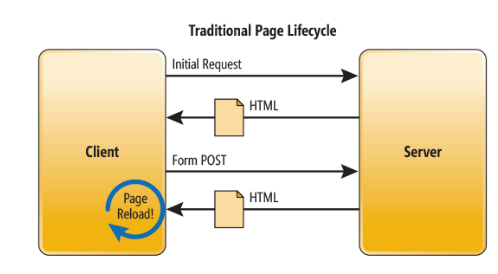
\includegraphics[width=.9\linewidth]{img/traditional_architecture.png}
\end{center}
\captionof{figure}{Traditional Architecture}\label{fig:traditional-architecture}
}
\subparagraph{The SPA architecture} \
\label{sec:orgfb2a92d}

{
\begin{center}
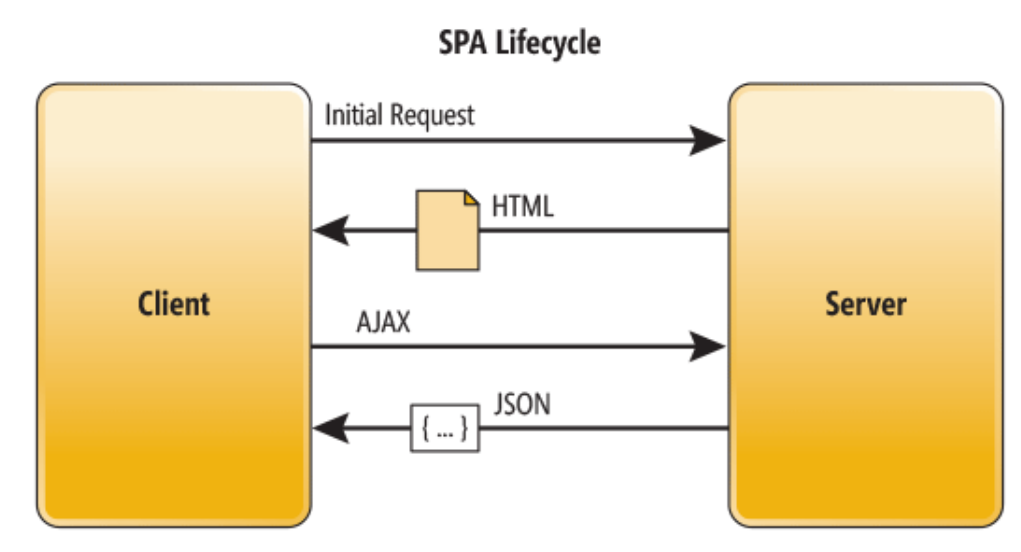
\includegraphics[width=.9\linewidth]{img/spa_architecture.png}
\end{center}
\captionof{figure}{SPA Architecture}\label{fig:spa-architecture}
}
\subparagraph{What are characteristics of an SPA?} \
\label{sec:org6d01651}
An SPA has the following properties:
\begin{itemize}
\item Plan HTML5 / CSS and JavaScript
\begin{itemize}
\item no plugins like SilverLight or Flash
\end{itemize}
\item no page reloads
\item Working Back-Button
\item Bookmarkable Links
\item Provides (limited) offline functionality
\item Uses (\href{../../../roam/20230108172748-what_is_rest.org}{REST})-API services for data access
\end{itemize}


{
\begin{center}
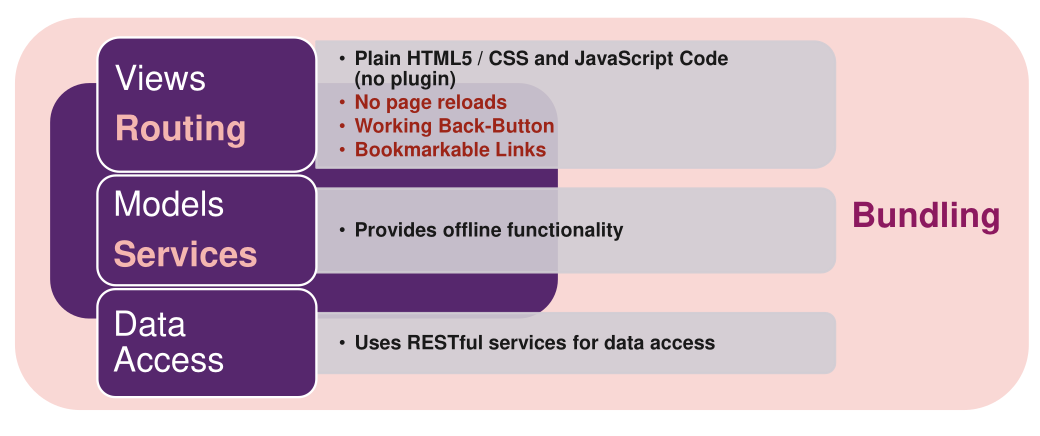
\includegraphics[width=.9\linewidth]{img/spa_logical_overview.png}
\end{center}
\captionof{figure}{Logical Overview of an SPA}\label{fig:logical-overview-of-an-spa}
}
\subparagraph{When would you prefer an SPA to a classic web application from the customer's point of view?} \
\label{sec:orgc2610cf}
\begin{quote}
As soon as a desktop (native) app with a similar user experience is required.
The page feels like an application.
An SPA also offers more options for complex web applications with lots of animations/graphical elements.
\end{quote}
\subparagraph{What do you see as the technical benefits of an SPA?} \
\label{sec:org2739fb8}

The server application is separated from the display by a structured interface (e.g. REST / ODATA / WSDL). This opens up various advantages:
\begin{itemize}
\item Seperation of Concerns
\item Better maintainability of the client code
\item Division into different teams / competence centers
\end{itemize}
\subparagraph{What does a typical layering in an SPA look like?} \
\label{sec:orga554ae6}
The Views are connected using a routing in the browser (no new request to the server).
The Business Logic provides data over servies and only the data layer will communicate directly with the server.

{
\begin{center}
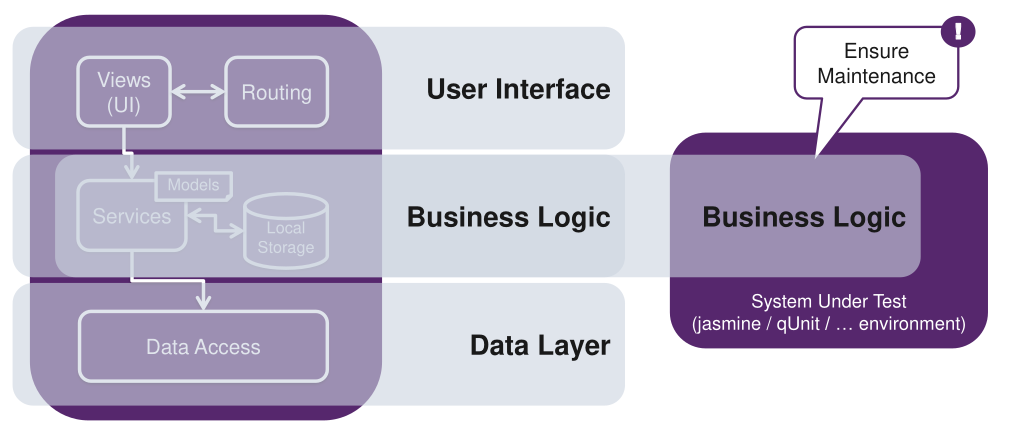
\includegraphics[width=.9\linewidth]{img/spa_layering.png}
\end{center}
\captionof{figure}{Layering in SPA}\label{fig:layering-in-spa}
}
\subparagraph{Why do we use bundling in an SPA?} \
\label{sec:org1ec5f76}
An SPA may consist of many single JS files, which may or may not dependt on each other.
To include them manually in your HTML is error pronce and tedious.

With bundling we achive the following things:
\begin{itemize}
\item All JS code must be delivered to the client over potentially metered/slow networks
\item Bundling and minifying the source leads to smaller SPA footprint (e.g. using \href{../../../roam/20231228113108-what_is_tree_shaking.org}{Tree Shaking})
\item Bundling leads to a reliable dependency management
\item Usage of pre and post processors during bundling
\end{itemize}


The initial footprint caused by bundling can be reduced by loading dependent modules on-demand.
\section{React}
\label{sec:orgd4c3a9d}
\subparagraph{What is JSX?} \
\label{sec:orga853850}
JSX is an extension to JavaScript.
It is used to write markup for an \href{../../../roam/20231228102611-what_is_a_single_page_application.org}{SPA}.
The JSX is transpiled during building into standard ECMAScript

\begin{quote}
JSX is an XML-like syntax extension to ECMAScript without any defined semantics.
It's NOT intended to be implemented by engines or browsers.
It's NOT a proposal to incorporate JSX into the ECMAScript spec itself.
It's intended to be used by various preprocessors (transpilers) to transform these tokens into standard ECMAScript. 
-- facebook.github.io/jsx/
\end{quote}
\subparagraph{How is JSX desugared in React?} \
\label{sec:org97bfab5}
\begin{listing}[htbp]
\begin{minted}[]{js}
import React from 'react'

function Container(props) {
  return
  className="container">
    {props.children}
  </div>
}
\end{minted}
\caption{\label{lst:jsx}JSX}
\end{listing}

\begin{listing}[htbp]
\begin{minted}[]{js}
function Container(props) {
  return React.createElement(
    "div",
    {className:"container"},
    props.children
  )
}
\end{minted}
\caption{\label{lst:desugared-jsx}Desugared JSX}
\end{listing}
\subparagraph{How do you make props available for all child components?} \
\label{sec:org0e1638c}
Some props must be availabel in all components (e.g. color scheme).
It does not scale well, if you have to pass all props from the root component.
To solve this problem, we can use contexts.
However, you should only use contexts for read-only variables and limit the number of different contexts.



\begin{minted}[]{js}
const themes = {
  light: {
    foreground: "#000000",
    background: "#eeeeee",
  },
  dark: {
    foreground: "#ffffff",
    background: "#222222",
  },
};
const ThemeContext = React.createContext(themes.light);

function App() {
  return (
    <ThemeContext.Provider value={themes.dark}>
      <Toolbar />
    </ThemeContext.Provider>
  );
}

function ThemedButton() {
  const theme = useContext(ThemeContext);
  return (
    <button style={{
              background: theme.background,
              color: theme.foreground }}>
      {" "}I am styled by theme context!{" "}
    </button>
  );
}
\end{minted}
\subparagraph{How does Redux work?} \
\label{sec:org90b38db}
The state in Redux is represented as trees of objects.
The tree is immutable.
When you change something in the tree, a new tree will be created (\href{../../../roam/20220616080932-functional_programming.org}{Functional Programming}).

A state action is communicated using a \emph{Redux Action}.
A \emph{Reducer} takes the action and the current state an applies the action on the state to generate a new state.

\begin{figure}[htbp]
\centering
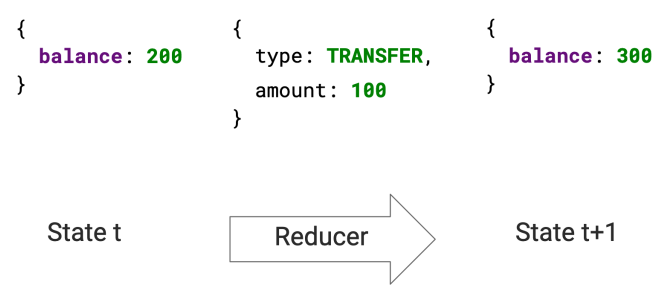
\includegraphics[width=.9\linewidth]{img/redux_action_reducer.png}
\caption{\label{fig:action-reducer-state-change}Action Reducer State change}
\end{figure}
\section{Angular}
\label{sec:org8b0d202}
\subparagraph{Angular} \
\label{sec:orgc799c9c}
Angular is a \href{../../../roam/20231228102611-what_is_a_single_page_application.org}{SPA} Framework:
\begin{itemize}
\item \href{../../../roam/20240108134405-typescript.org}{TypeScript} based
\item Reduces boilerplate code
\item Comes with a \href{../../../roam/20200904154006-dependency_injection.org}{Dependency Injection} mechanism
\item Provides fast, JS-optimized 2-way binding
\item Clearly structured, supports information hiding principle on multiple levels of abstraction
\item Increases the testability and maintainability of the client-side code
\item Provides a framework that covers a wide range of topics from templating to data-services
− but doesn’t exactly specify how to wire them
\end{itemize}

\begin{quote}
Angular is an advanced SPA framework…
…which allows you to use the latest web engineering principles.
\end{quote}
\subparagraph{Angular Architectural Parts} \
\label{sec:orga17d027}
\begin{description}
\item[{ngModules}] A cohesive block of code dedicated to closely related set of capabilities
\item[{directives}] Provides instructions to transform the DOM
\item[{components}] A component is a directive-with-a-template; it controls a section of the view
\item[{templates}] A template is a form of HTML that tells Angular how to render the component
\item[{metadata}] Metadata describes a class and tells Angular how to process it
\item[{services}] Provides logic of any value, function, or feature that your application needs
\end{description}
\subparagraph{Angular Module Declaration} \
\label{sec:org4b161d5}
\begin{itemize}
\item declarations: View Classes that belongs to this module
\item exports: Subset of declarations that should be visible in other modules
\item imports: Modules should be imported into this module
\item providers: Creators of services that this module contributes to the global DI container
\item bootstrap: Main application view (only in root module)
\end{itemize}
\subparagraph{Binding Syntax} \
\label{sec:org5dba381}
\begin{listing}[htbp]
\begin{minted}[]{html}
<!-- Two Way Binding -->
<input type="text" [(ngModel)]="counter.team">

<!-- One Way (View to Model) -->
<button (click)="counter.eventHandler($event)">

<!-- One Way (Model to View) -->
<p>{{counter.team}}</p>
\end{minted}
\caption{\label{lst:bindings-variants-in-angular}Bindings variants in Angular}
\end{listing}
\subparagraph{Directives} \
\label{sec:org3a1c7bf}
Similar to a component, but without a template.
Declared as a TypeScript class with an \texttt{@Directive()} function decorator.
\begin{itemize}
\item \textbf{Structural} directive: modifies structure of DOM
\begin{itemize}
\item \texttt{*ngIf}
\item \texttt{*ngFor}
\end{itemize}
\item \textbf{Attribute} directive: alters appereance / behavior of an existing element
\begin{itemize}
\item \texttt{[ngStyle]}
\item \texttt{[ngClass]}
\end{itemize}
\end{itemize}
\subparagraph{Services} \
\label{sec:org5a5a4de}
Provides any value, function, or feature that your application needs.
Almost anything can be a service - it should do one thing and do it well.

The \texttt{@Injectable} decorater is used to register the service in the DI container.
\texttt{@Injectable(\{ providedIn: 'root' \})export class CounterService \{\}}
\subparagraph{Forms} \
\label{sec:orgbf093c1}

{
\begin{minted}[]{html}
<form (ngSubmit)="doLogin(sampleForm)" #sampleFrom="ngForm">
  <button type="submit" [disabled]="!sampleForm.form.valid">Submit</button>
</form>
\end{minted}
\captionof{listing}{Angular Form Markup}\label{lst:angular-form-markup}
}

{
\begin{minted}[]{typescript}
@Component({})
export class SampleComponent {
  public doLogin(f?: NgForm): boolean {
    if (f?.form.valid) { /* do stuff */ return true; }
    return false;
  }
}
\end{minted}
\captionof{listing}{Angular Form Logic}\label{lst:angular-form-logic}
}
\subparagraph{Component Lifecycle\hfill{}\textsc{ATTACH}} \
\label{sec:orgf16968a}
{
\begin{center}
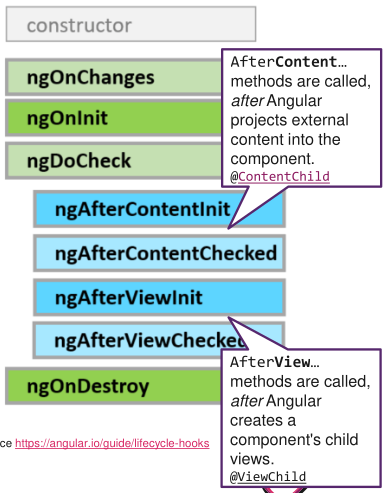
\includegraphics[width=.9\linewidth]{img/component_lifecycle.png}
\end{center}
\captionof{figure}{Component Lifecycle}\label{fig:component-lifecycle}
}
\subparagraph{Asynchronous Services} \
\label{sec:org90e1388}
Do not use RxJS in the UI.
It is sufficient to use \texttt{EventEmitter}
\subparagraph{RxJS} \
\label{sec:org1a53b43}
\subparagraph{Routing} \
\label{sec:org89333ea}
\begin{description}
\item[{\texttt{.forRoot()}}] use EXACTLY once to declare routes on root (top) level
\item[{\texttt{.forChild()}}] use when declaring sub-routings (on all sub-levels)
\end{description}
\subparagraph{Module Type / Example Architecture} \
\label{sec:org807bb38}
\begin{description}
\item[{Root / App Module}] provies the entry point for the app
\item[{Feature Modules}] clear boundaries between the application features
\item[{Shared Module}] Holds common components / directives / pipes
\item[{Core Module}] Keeps your Root Module clean
\end{description}
\subparagraph{Feature Module (sub) Types} \
\label{sec:orgd654b4f}
\begin{description}
\item[{Domain Modules}] deliver a UI dedicated to a particular application domain
\item[{Routing Modules}] specifies the routing specific configuration settings of the Feature (or Root) Module
\item[{Service Modules}] provides utility services such as data access and messaging
\item[{Widget Modules}] makes components, directives, and pipes available to external modules
\item[{Lazy Modules (Routed Modules)}] represents lazily loaded Feature Modules.
\end{description}
\subparagraph{RxJS - Observable Types} \
\label{sec:orgad1f940}
\begin{description}
\item[{Hot Observables}] Sequence of events (such as mouse move events or stock tickers)
\item[{Cold Observables}] Observables start running on subscription (such as async web requests) and complete automatically
\end{description}
\subparagraph{Flux Architecture} \
\label{sec:org59931ef}
The state in Redux is represented as trees of objects.
The tree is immutable.
When you change something in the tree, a new tree will be created (\href{../../../roam/20220616080932-functional_programming.org}{Functional Programming}).

A state action is communicated using a \emph{Redux Action}.
A \emph{Reducer} takes the action and the current state an applies the action on the state to generate a new state.

{
\begin{center}
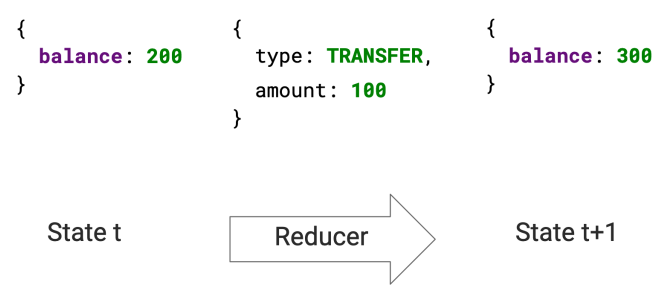
\includegraphics[width=.9\linewidth]{img/redux_action_reducer.png}
\end{center}
\captionof{figure}{Action Reducer State change}\label{fig:action-reducer-state-change}
}
\subparagraph{Pipes} \
\label{sec:org2044586}
\begin{description}
\item[{Pure Pipes}] Pure pipes are executed when it detects a ‘pure change’ to the input expression (DatePipe)
\item[{Impure Pipes}] Impure pipes are executed on every component change detection cycle (AsyncPipe)
\end{description}
\section{ASP.NET}
\label{sec:org67123a9}
\subparagraph{PWA} \
\label{sec:org89a3753}
\begin{itemize}
\item \href{../../../roam/20240108155002-pwa.org}{PWA}
\end{itemize}
\subparagraph{For what is Firbase used?} \
\label{sec:orga07f33f}
To develop a PWA we used the following features from Firebase:
\begin{itemize}
\item Cloud Firestore / Realtime (DB)
\item Cloud Functions (Serverless Functions)
\item Authentication
\item Hosting / Cloud Storage
\end{itemize}
\subparagraph{Front Controller} \
\label{sec:orgb610e9d}
The Front Controller is the Entry Point and executes logging and routing (actions that are required for all incoming requiest).
After that, the front controller forwards the request the the responsible controller.
\subparagraph{MVVM} \
\label{sec:org24d67e3}
\begin{itemize}
\item \href{../../../roam/20211103140901-mvvm.org}{MVVM}
\end{itemize}
\subparagraph{Middleware} \
\label{sec:org7a32bef}
\begin{description}
\item[{source}] \url{https://learn.microsoft.com/en-us/aspnet/core/fundamentals/middleware/?view=aspnetcore-8.0}
\end{description}
Middleware is a "function block" and has a certain task.
When a middleware has finished its task it will call the next following middleware or finishes the request.

Using \texttt{app.Run()} a terminating middleware is registerd.
After this middleware the request is finished.
\begin{minted}[]{csharp}
app.Run(async (context) => {
    await context.Response.WriteAsync("Hello");

    app.Run();
});
\end{minted}

Context contains all information for the request as well for the response.
Using \texttt{app.Use(<lambda>)} a middleware is registred, that calls the next middleware (does not terminate)
\begin{minted}[]{csharp}
app.Use(async (context, next) => {
    await context.Response.WriteAsync("Hello");    
    next.Invoke();
});

app.Use(async (context, next) => {
    await context.Response.WriteAsync(" Welt");    
    next.Invoke();
});

app.Run();
\end{minted}

Extension Method as middleware
\begin{minted}[]{csharp}
// Extension Method als Middleware
app.UseMyMiddlware();


app.Run();


static class MyMiddlwares
{
    public static IApplicationBuilder UseMyMiddlware(this WebApplication app)
    {
        return app.Use(async (context, next) =>
        {
            await context.Response.WriteAsync(", Hello from Extension Method");
            await next.Invoke();
        });
    }
}
\end{minted}

Class as middleware.
Is often used when the middlware becomes larger than 2-3 lines of code.
\begin{minted}[]{csharp}
app.UseMiddleware<MyClassMiddleware>();

app.Run();

class MyClassMiddleware
{
    private readonly RequestDelegate _next;
    public MyClassMiddleware(RequestDelegate next)
    {
        if (next == null)
            throw new ArgumentNullException(nameof (next));

        this._next = next;
    }

    public async Task InvokeAsync(HttpContext context)
    {
        await context.Response.WriteAsync(", Hello from Middleware class");
        await this._next.Invoke(context);
    }
}
\end{minted}
\subparagraph{Middleware Registration} \
\label{sec:org25abf62}
\begin{itemize}
\item \texttt{app.Use()}
\item \texttt{app.Map()}
\item \texttt{app.Run()}
\item \texttt{app.UseMiddleware<>()}
\end{itemize}
\subparagraph{Dependency Injection - Lifetime} \
\label{sec:orgeae8a0f}
Register services with different lifetimes:
\begin{itemize}
\item Transient, are created every time when used
\item Scoped, are created once for every request (used most often)
\item Singelton, it's just a singelton (only for Readonly, configs, options)
\end{itemize}


Register a transient service: \texttt{builder.Services.AddTransient<>()}


\textbf{Captive dependency}
The term "captive dependency" refers to the misconfiguration of service lifetimes, where a longer-lived service holds a shorter-lived service captive.
\begin{itemize}
\item Transient requires Singelton -> OK
\item Singelton requires Transient -> Not OK
\begin{itemize}
\item When the singleton is used a 2nd time (e.g. parallel) it uses the same reference to the transient service.
\item Transient services are normally \textbf{NOT} thread-safe and an error can occuer when used in a not thread safe context
\end{itemize}
\end{itemize}
\subparagraph{Entity Framework} \
\label{sec:org4d656f1}
\begin{itemize}
\item \href{../../../roam/20220108180326-entity_framework.org}{Entity Framework}
\end{itemize}
\subparagraph{Web Assembly File Type} \
\label{sec:org28ec2a7}
\begin{itemize}
\item *.WASM (WebAssembly)
\begin{itemize}
\item Compiled Web Assembly
\item Can be transformed back to WAT
\end{itemize}

\item *.WAT
\begin{itemize}
\item Text Based Web Assembly
\item Can be compiled to WASM
\end{itemize}

\item Web Assembly
\begin{itemize}
\item Is a stack machine (similar to the JVM)
\item \href{../../../roam/20221230171752-what_is_a_evaluation_stack.org}{Evaluation Stack}
\end{itemize}
\end{itemize}
\subparagraph{Key Concepts} \
\label{sec:orgafff8b6}
\begin{itemize}
\item Module
\begin{itemize}
\item Represents a WebAssembly binary that has been compiled by the browser into executable machine code
\item Stateless
\item Import / Export
\end{itemize}
\item Memory
\begin{itemize}
\item shared memory section between JS and web assembly
\end{itemize}
\item Table
\begin{itemize}
\item A resizable typed array of references (e.g. to functions) that could not otherwise be stored as raw bytes in Memory (for safety and portability reasons).
\end{itemize}
\item Instance
\begin{itemize}
\item A Module paired with all the state it uses at runtime including a Memory, Table, and set of imported values.
\end{itemize}
\end{itemize}


\end{multicols}
\end{document}
